\documentclass[12pt,hyperref,a4paper,UTF8]{ctexart}
\usepackage{HDUReport}
\usepackage{listings}
\usepackage{xcolor}
\usepackage{graphicx}
\usepackage{setspace}
\usepackage{float}
\setstretch{1.5} % 设置全局行距为1.5倍

\usepackage{enumitem} % 载入enumitem包以便自定义列表环境
\setlist[itemize]{itemsep=0pt, parsep=0pt} % 设置itemize环境的项目间距和段落间距

\setmainfont{Times New Roman} % 英文正文为Times New Roman


\usepackage{tikz}
\usetikzlibrary{shapes.geometric, arrows}
\usetikzlibrary{positioning, arrows.meta}
\usetikzlibrary{calc}


% 设置MATLAB代码样式
\definecolor{codegreen}{rgb}{0,0.6,0}
\definecolor{codegray}{rgb}{0.5,0.5,0.5}
\definecolor{codepurple}{rgb}{0.58,0,0.82}
\definecolor{backcolour}{rgb}{0.95,0.95,0.92}

\lstdefinestyle{matlab}{
    backgroundcolor=\color{backcolour},   
    commentstyle=\color{codegreen},
    keywordstyle=\color{magenta},
    numberstyle=\tiny\color{codegray},
    stringstyle=\color{codepurple},
    basicstyle=\ttfamily\small,
    breakatwhitespace=false,         
    breaklines=true,                 
    captionpos=b,                    
    keepspaces=true,                 
    numbers=left,                    
    numbersep=5pt,                  
    showspaces=false,                
    showstringspaces=false,
    showtabs=false,                  
    tabsize=2,
    frame=single,
    language=Matlab
}
%封面页设置
{   
    %标题
    \title{ 
        \vspace{1cm}
        \heiti \Huge \textbf{《数字信号处理课程设计》实验报告} \par
        \vspace{1cm} 
        \heiti \Large {\underline{实验报告4:用窗口法/频率采样法设计FIR数字滤波器}   } 
        \vspace{3cm}
    
    }

    \author{
        \vspace{0.5cm}
        \kaishu\Large 学院\ \dlmu[9cm]{卓越学院} \\ %学院
        \vspace{0.5cm}
        \kaishu\Large 学号\ \dlmu[9cm]{23040447} \\ %班级
        \vspace{0.5cm}
        \kaishu\Large 姓名\ \dlmu[9cm]{陈文轩} \qquad  \\ %学号
        \vspace{0.5cm}
        \kaishu\Large 专业\ \dlmu[9cm]{智能硬件与系统(电子信息工程)} \qquad \\ %姓名 
    }
        
    \date{\today} % 默认为今天的日期,可以注释掉不显示日期
}
%%------------------------document环境开始------------------------%%
\begin{document}

%%-----------------------封面--------------------%%
\cover
\thispagestyle{empty} % 首页不显示页码
%%------------------摘要-------------%%
%\newpage
%\begin{abstract}




%\end{abstract}

%\thispagestyle{empty} % 首页不显示页码

%%--------------------------目录页------------------------%%
% \newpage
% \tableofcontents
% \thispagestyle{empty} % 目录不显示页码

%%------------------------正文页从这里开始-------------------%
\newpage
\setcounter{page}{1} % 让页码从正文开始编号

%%可选择这里也放一个标题
%\begin{center}
%    \title{ \Huge \textbf{{标题}}}
%\end{center}
\section{实验目的}

了解一个实际滤波器设计过程,加深掌握用窗口法设计FIR滤波器的原理和窗函数对
滤波器性能的影响。并掌握频率采样设计法,加深过渡点对滤波器性能的影响。

\section{实验基本原理}

\subsection{窗口法}

窗口法是一种常用的FIR数字滤波器设计方法。其基本思想是:首先得到理想频率响应 $H_d(e^{j\omega})$ 对应的理想单位脉冲响应 $h_d(n)$,通常情况下 $h_d(n)$ 是无限长的。为了得到实际可实现的FIR滤波器,需要将 $h_d(n)$ 截断为有限长度 $N$,并乘以一个窗函数 $w(n)$,得到实际的滤波器单位脉冲响应 $h(n)$。

$$h(n) = h_d(n) \cdot w(n)$$

其中,$w(n)$ 是窗函数,常见的窗函数包括矩形窗、汉宁窗、汉明窗、布莱克曼窗等。不同的窗函数具有不同的时域和频域特性,选择合适的窗函数可以有效地控制滤波器的过渡带宽度、阻带衰减等性能指标。例如,矩形窗的定义如下:

$$ w(n) = \begin{cases} 
1, & 0 \leq n \leq N-1 \\
0, & \text{otherwise}
\end{cases} $$

加窗的作用是减小截断带来的频谱泄漏和旁瓣效应,从而改善滤波器的实际性能。窗口法设计步骤简明,计算量小,适用于对滤波器性能要求不是特别苛刻的场合。

\subsection{频率采样法}

频率采样法是另一种FIR数字滤波器设计方法。其基本思想是:首先在单位圆上选取 $N$ 个等间隔的频率采样点 $\omega_k = \frac{2\pi}{N}k, \quad k = 0, 1, \dots, N-1$,直接指定这些频率点上的理想频率响应值 $H(k)$。然后通过离散傅里叶反变换(IDFT)计算出滤波器的单位脉冲响应 $h(n)$:

$$ h(n) = \frac{1}{N} \sum_{k=0}^{N-1} H(k) e^{j\frac{2\pi}{N}kn}, \quad n = 0, 1, \dots, N-1 $$

其中,$H(k)$ 是在频率采样点 $\omega_k$ 上的频率响应值。为了保证 $h(n)$ 是实数,需要满足共轭对称性,即 $H(k) = H^* (N-k)$。

该方法适用于设计具有特殊频率响应的滤波器,尤其是当理想频率响应在某些频率点上已知时。频率采样法可以灵活地控制滤波器在特定频率点的响应,但在频率点之间的响应可能不够理想,因此常结合插值或窗函数进一步优化。

\section{实验要求及内容}

\subsection{窗口法}

用改进余弦窗设计一个 FIR 线性相应相位低通数字滤波器,已知 \(o_c = 0.5 \pi, N = 21\) 。编写调试程序,要求在幕幕上显示出单位脉冲响应 \(h(n)\) 的数值,画出其幅度响应 \(\left| H(e^{j\theta}) \right|\) 的曲线。

\subsection{频率采样法}
实验前,学生应复习用频率采样法设计FIR 滤波器的基本原理,预习实验指导书。

2、编写好一个设计线性相位 FIR 高通滤波器,\(\alpha_c = 0.8\pi\),\(N = 64\) 的程序。要求在屏幕上打印出 \(h(n)\) 值,画出 \(\left|H(e^{i\omega})\right|\) 曲线。

3、实验时,设置 \(0\) 个过渡点,一个过渡点和二个过渡点,比较设计所得的 \(\left|H(e^{i\omega})\right|\) 曲线。

4、实验后,学生对结果作出解释,写好实验报告。

\section{实验结果与分析}

\subsection{窗口法题目}

% 插入MATLAB代码
\begin{lstlisting}[style=matlab, caption={实验一MATLAB实现代码}]
% 定义FIR低通滤波器的设计参数
Fs = 720;        % 采样频率 (Hz)
N = 21;          % 滤波器阶数
wc = 0.537 * pi;   % 归一化截止频率 (0.5π)

% 设计FIR低通滤波器(Hamming窗)
b = fir1(N, wc/pi);
a = 1;

% 计算频率响应
[H, W] = freqz(b, a, 1024);
freq_normalized = W/pi;  % 归一化频率(0~1)

% 精确找到截止频率对应的索引
[~, idx_wc] = min(abs(W - wc));
H_wc = H(idx_wc);  % 该频率点的复频响应

% ===== 专业绘图 =====
figure('Position', [100 100 900 800]);

% 1. 幅频特性(线性)
subplot(3,2,1);
plot(freq_normalized, abs(H), 'b', 'LineWidth', 1.5);
hold on;
% 精确标定截止频率点(红色圆点落在曲线上)
plot(freq_normalized(idx_wc), abs(H_wc), 'ro', 'MarkerFaceColor', 'r', 'MarkerSize', 8);
text(freq_normalized(idx_wc), abs(H_wc), ...
    sprintf(' (%.2fπ, %.3f)', freq_normalized(idx_wc), abs(H_wc)), ...
    'VerticalAlignment', 'bottom', 'HorizontalAlignment', 'right');
title('幅频特性(线性)');
xlabel('归一化频率 (\times\pi rad/sample)');
ylabel('幅度');
grid on;
xlim([0 1]);

% 2. 幅频特性(dB)
subplot(3,2,2);
plot(freq_normalized, 20*log10(abs(H)), 'b', 'LineWidth', 1.5);
hold on;
% 精确标定截止频率点
plot(freq_normalized(idx_wc), 20*log10(abs(H_wc)), 'ro', 'MarkerFaceColor', 'r', 'MarkerSize', 8);
text(freq_normalized(idx_wc), 20*log10(abs(H_wc)), ...
    sprintf(' (%.2fπ, %.1f dB)', freq_normalized(idx_wc), 20*log10(abs(H_wc))), ...
    'VerticalAlignment', 'bottom', 'HorizontalAlignment', 'right');
title('幅频特性(dB)');
xlabel('归一化频率 (\times\pi rad/sample)');
ylabel('幅度 (dB)');
grid on;
xlim([0 1]);
ylim([-80 5]);

% 3. 相位响应(解卷绕)
subplot(3,2,3);
phase = unwrap(angle(H));
plot(freq_normalized, phase, 'm', 'LineWidth', 1.5);
hold on;
% 标定截止频率相位
plot(freq_normalized(idx_wc), phase(idx_wc), 'ro', 'MarkerFaceColor', 'r', 'MarkerSize', 8);
title('相位响应');
xlabel('归一化频率 (\times\pi rad/sample)');
ylabel('相位 (rad)');
grid on;
xlim([0 1]);



% 5. 单位脉冲响应
subplot(3,2,[5 6]);
stem(0:N, b, 'filled', 'LineWidth', 1.5, 'MarkerSize', 5);
title('单位脉冲响应 h(n)');
xlabel('采样点 n');
ylabel('幅度');
grid on;

% 显示关键参数
disp(['截止频率: ', num2str(wc/pi), 'π (', num2str(wc*Fs/(2*pi)), ' Hz)']);
disp(['-3dB点实际增益: ', num2str(20*log10(abs(H_wc))), ' dB']);
disp(['群延迟(理论N/2): ', num2str(mean(group_delay(1:idx_wc_gd))), ' 采样点']);


\end{lstlisting}



\begin{figure}[H] % [H] 表示强制当前位置插入
        \centering
        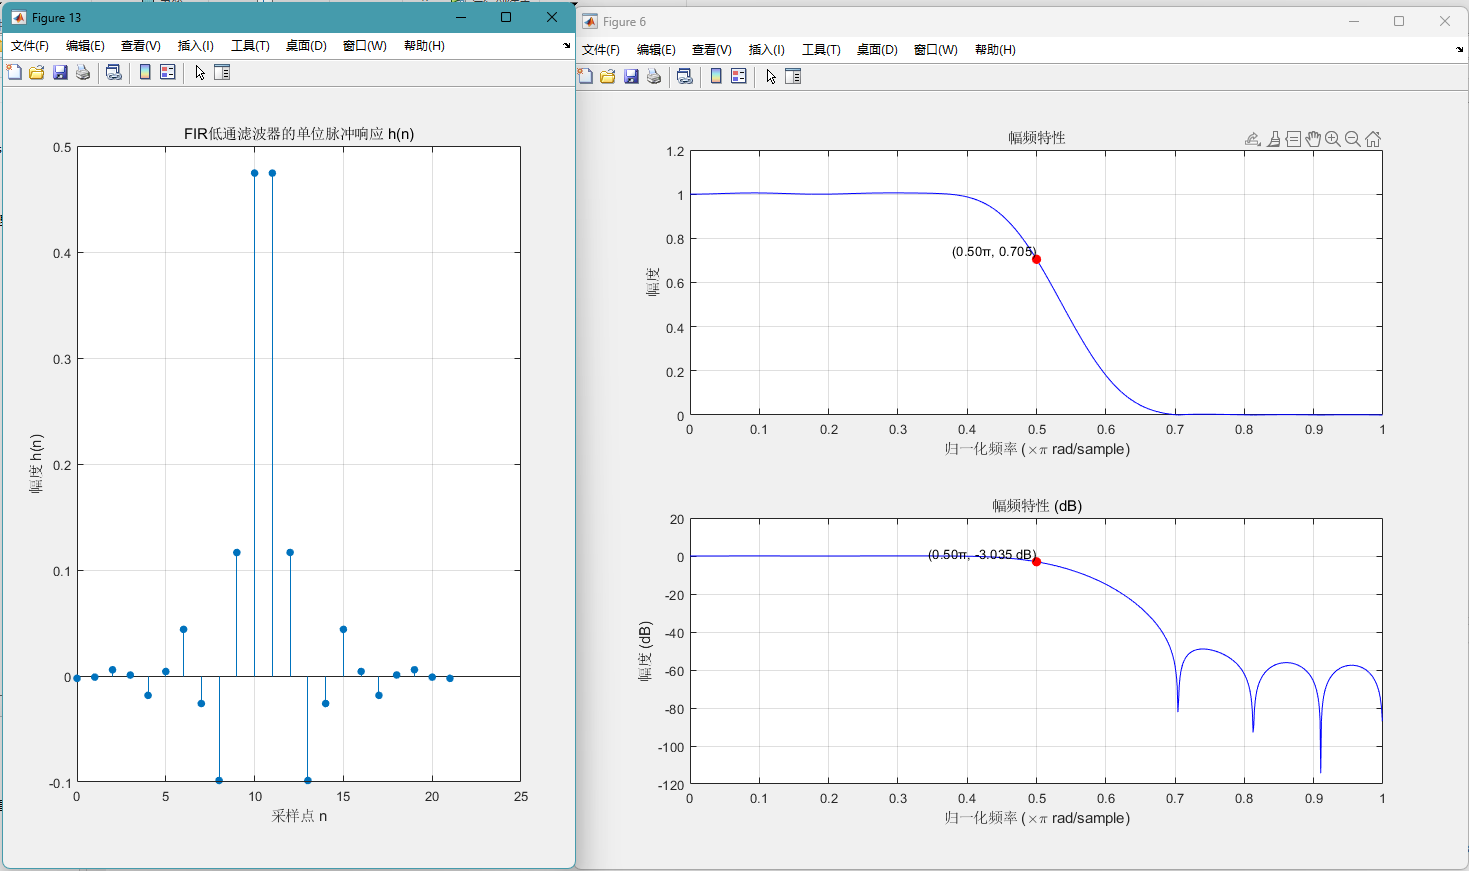
\includegraphics[width=0.9\textwidth]{figures/304.png} % 调整宽度为文本宽度的 80%
        \caption{matlab绘图} %图片标题
        \label{fig:example} % 图片标签,用于引用
\end{figure}

\begin{figure}[H] % [H] 表示强制当前位置插入
        \centering
        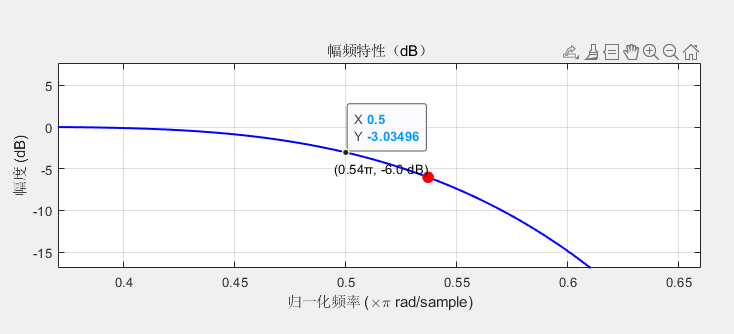
\includegraphics[width=0.9\textwidth]{figures/305.png} % 调整宽度为文本宽度的 80%
        \caption{matlab绘图} %图片标题
        \label{fig:example} % 图片标签,用于引用
\end{figure}



\subsection{频率采样法题目一}


% 插入MATLAB代码
\begin{lstlisting}[style=matlab, caption={ MATLAB实现代码}]


\end{lstlisting}

\begin{table}[H]
\centering
\caption{题目二滤波器系数}
\label{tab:filter_coef2}
\begin{tabular}{|c|c|c|c|}
\hline
\textbf{系数类型} & \multicolumn{3}{c|}{\textbf{系数值}} \\
\hline
\textbf{滤波器阶数} & \multicolumn{3}{c|}{N = 2} \\
\hline
\textbf{分子系数} & 0.0778 & -0.1556 & 0.0778 \\
\hline
\textbf{分母系数} & 1.0000 & 1.0708 & 0.3821 \\
\hline
\end{tabular}
\end{table}

\begin{figure}[H] % [H] 表示强制当前位置插入
        \centering
        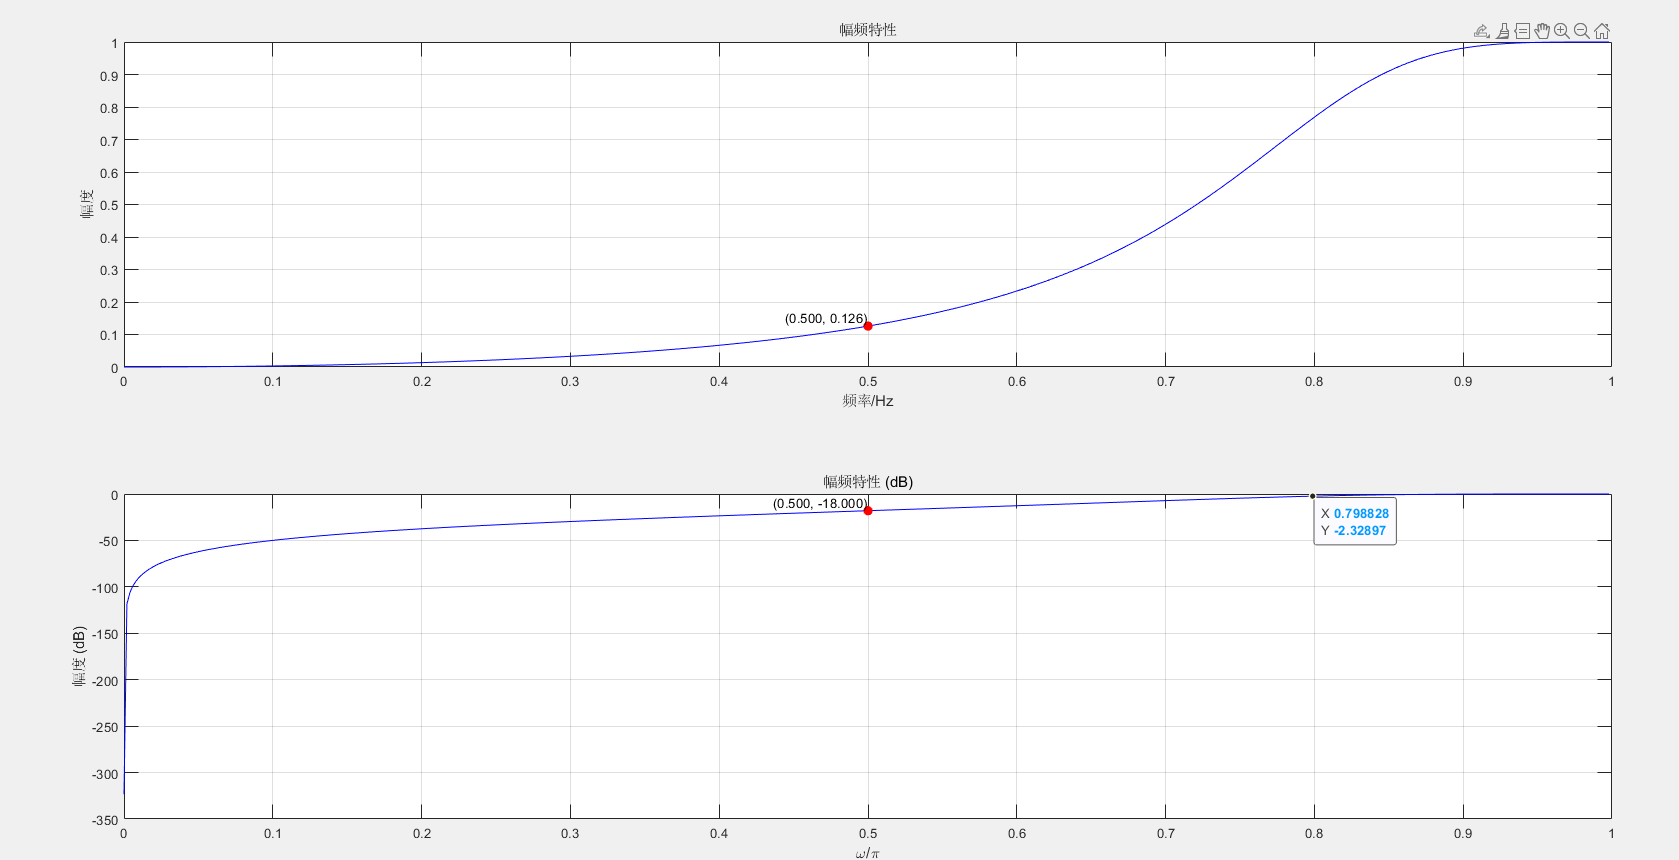
\includegraphics[width=0.9\textwidth]{figures/302.png} % 调整宽度为文本宽度的 80%
        \caption{matlab绘图} %图片标题
        \label{fig:example} % 图片标签,用于引用
\end{figure}

\subsection{题目三}


% 插入MATLAB代码
\begin{lstlisting}[style=matlab, caption={ MATLAB实现代码}]


\end{lstlisting}

\begin{table}[H]
\centering
\caption{题目三滤波器系数}
\label{tab:filter_coef3}
\begin{tabular}{|c|c|c|c|c|c|c|c|}
\hline
\textbf{系数类型} & \multicolumn{7}{c|}{\textbf{系数值}} \\
\hline
\textbf{分子系数} & 0.3642 & 0.0000 & -1.0926 & -0.0000 & 1.0926 & 0.0000 & -0.3642 \\
\hline
\textbf{分母系数} & 1.0000 & -0.0000 & -1.1162 & 0.0000 & 0.6676 & -0.0000 & -0.1299 \\
\hline
\end{tabular}
\end{table}

\begin{figure}[H] % [H] 表示强制当前位置插入
        \centering
        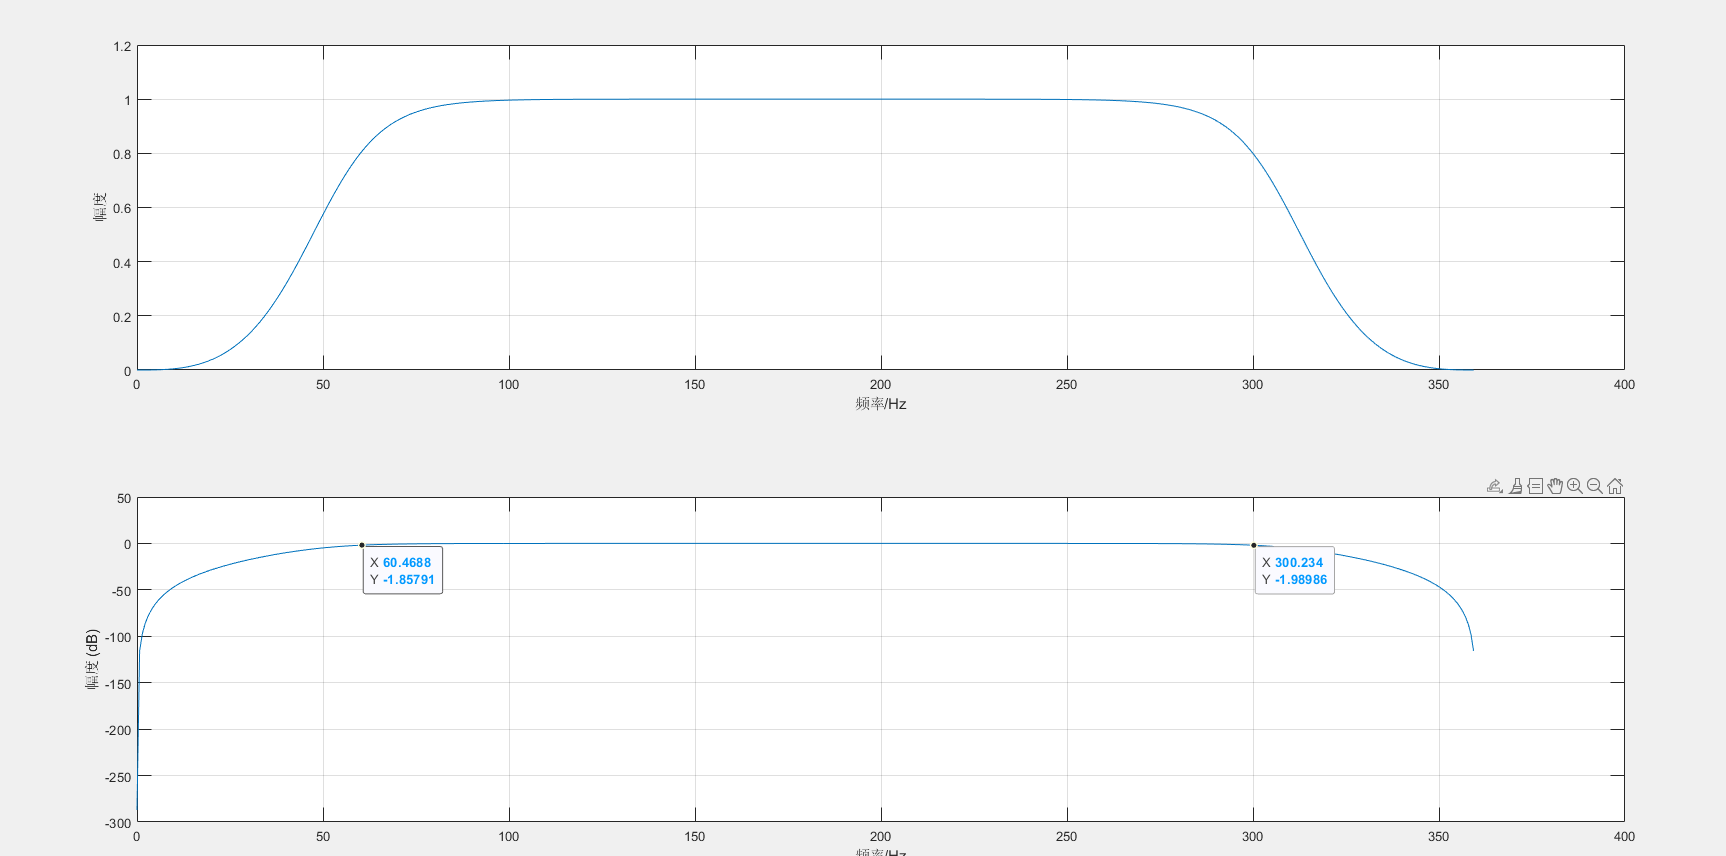
\includegraphics[width=0.9\textwidth]{figures/303.png} % 调整宽度为文本宽度的 80%
        \caption{matlab绘图} %图片标题
        \label{fig:example} % 图片标签,用于引用
\end{figure}



\section{实验小结}

本次实验系统地学习并实践了双线性变换法设计IIR数字滤波器的全过程,主要包括低通、高通和带通巴特沃斯滤波器的设计与分析。通过MATLAB编程实现,掌握了从设计指标出发,经过预扭曲、模拟滤波器设计、双线性变换到数字滤波器实现的完整流程。实验结果表明,所设计的滤波器均能较好地满足幅频特性要求,且通过表格清晰展示了各滤波器的分子、分母系数,便于后续实现和分析。

本实验的主要收获如下:

\begin{itemize}
    \item 熟悉了双线性变换的基本原理及其在数字滤波器设计中的应用,理解了频率预扭曲的重要性。
    \item 掌握了MATLAB中巴特沃斯滤波器的阶数计算、系数求解及频率响应绘制方法。
    \item 通过对比不同类型和参数的滤波器,直观体会了参数变化对滤波器性能的影响。
    \item 学会了如何规范地整理和展示滤波器系数,提升了实验报告的规范性和可读性。
\end{itemize}

本次实验不仅加深了对数字信号处理理论的理解,也提升了实际工程实现能力,为后续更复杂的信号处理任务打下了坚实基础。

\end{document}